\documentclass[9pt,a4paper]{extarticle}


	\usepackage[margin=5em,bottom=8em]{geometry}


%1 est la marge gauche
%2 est la marge en haut
%3 est la marge droite
%4 est la marge en bas
%5 fixe la hauteur de l'entête
%6 fixe la distance entre l'entête et le texte
%7 fixe la hauteur du pied de page
%8 fixe la distance entre le texte et le pied de page
%------------------------------Packages généraux------------------------------

\usepackage[english]{babel}
\usepackage[T1]{fontenc}
\usepackage{ae}
\usepackage[utf8]{inputenc}
\usepackage{scrextend}
\usepackage{hyperref}
 \hypersetup{
    colorlinks = true,
    linkcolor=black,
    urlcolor = black
    }
%-------------------------Mathématiques------------------------------
\usepackage{amsmath}
\usepackage{amssymb}
\usepackage{amsthm}
\usepackage{amsfonts}
\usepackage{eucal}
\newcommand\independent{\protect\mathpalette{\protect\independenT}{\perp}}
\def\independenT#1#2{\mathrel{\rlap{$#1#2$}\mkern2mu{#1#2}}}
%-----------------------Codes et algorithmes--------------------------
\usepackage{algorithm}
%\usepackage{algorithmic}
%\usepackage{clrscode3e}
\usepackage[noend]{algpseudocode}
%\newcommand{\pushline}{\Indp}% Indent
%\newcommand{\popline}{\Indm\dosemic}% Undent
%\newcommand{\nonl}{\renewcommand{\nl}{\let\nl\oldnl}}%


%------------------------------Graphics------------------------------

\usepackage{graphicx}
\usepackage{fancyhdr}
\usepackage{fancybox}
\usepackage{color}
\usepackage{pgf, tikz}
\usetikzlibrary{arrows, automata}
%\usepackage{slashbox}

%------------------Sub-sections--------%
\usepackage{titlesec}
\usepackage{hyperref}
\usepackage{comment}
\usepackage{qrcode}

\usepackage{hyperref}
               
 \hypersetup{
    colorlinks = true,
    linkcolor=black,
    urlcolor = black
    }
    
\newenvironment{solution}
    {%\begin{center}
    %\begin{tabular}{|p{0.9\textwidth}|}
    %\hline\\
    \color{red}
    }
    { 
    %\\\\\hline
    %\end{tabular} 
    %\end{center}
    \color{black}
    }
    
\newcommand{\blue}[1]{\textcolor{blue}{#1}}


\newif\ifhideproofs
\hideproofstrue %uncomment to hide proofs

\ifhideproofs
\usepackage{environ}
\NewEnviron{hide}{}
\let\solution\hide
\let\endsolution\endhide
\fi

\title{{\bf INFO8006 Introduction to Artificial Intelligence}\\[1em]
Exercises 2: Constraint satisfaction problems}
\date{}
%------------------------------Début du document------------------------------
\begin{document}
\maketitle
\vspace{-4em}
%------------------------------Page de garde------------------------------

  \section*{Learning outcomes}
  At the end of this exercise session you should be able to:
  \begin{itemize}
       \item define a search problem as a constraint satisfaction problem (CSP).
       \item draw the constraint graph of a CSP.
       \item define what backtracking is and know how to use it.
       \item define and apply variable and value ordering.
       \item understand the syntax and the semantic of propositional logic.
       \item check the entailment of two propositions.
       \item show how a SAT problem can be formulated as a CSP.
       
   \end{itemize}
   \section*{Exercise 1: 8 Queens}
   \textit{The eight queens puzzle is the problem of placing eight chess queens on an $8\times8$ chessboard so that no two queens threaten each other. Thus, a solution requires that no two queens share the same row, column, or diagonal. The eight queens puzzle is an example of the more general n queens problem of placing n non-attacking queens on an $n\times n$ chessboard, for which solutions exist for all natural numbers n with the exception of n=2 and n=3.}%\footnote{\url{https://en.wikipedia.org/wiki/Eight\_queens\_puzzle}}
   Consider the case where the chessboard size $n = 4$. Answer the following questions:
   \begin{enumerate}
       \item Define the problem as a CSP (implicit constraints are allowed). 
    \begin{solution}
    \\
     A CSP is defined by a set of variables and their domains plus a set of constraints involving these variables.
     Let the tuples of variables $\{x_i, y_i\} \in \{1,..,4\}\times \{1,..,4\}$, where  $i\in \{1,..,4\}$ represents the position of the queen $i$.
     We have the following constraints:
     \begin{itemize}
         \item $x_i \neq x_j \forall i, j \in \{1,..,4\} \text{ and } i \neq j$
 , they represent the column constraints.
 		\item $y_i \neq y_j \forall i, j \in \{1,..,4\} \text{ and } i \neq j$ , they represent the row constraints.
         \item $\{x_i+k, y_i+k\} \neq \{x_j, y_j\} \forall i, j, k \in \{1,..,4\} \text{ and } i \neq j$
         \item $\{x_i-k, y_i+k\} \neq \{x_j, y_j\} \forall i, j, k \in \{1,..,4\} \text{ and } i \neq j$
         \item $\{x_i-k, y_i-k\} \neq \{x_j, y_j\} \forall i, j, k \in \{1,..,4\} \text{ and } i \neq j$
         \item $\{x_i+k, y_i-k\} \neq \{x_j, y_j\} \forall i, j, k \in \{1,..,4\} \text{ and } i \neq j$,  they represent the diagonal constraints.
     \end{itemize}
     \end{solution}
       \item Draw the graph of constraints from your CSP formulation.
       \begin{solution}
       \\
       The graph of constraints is a complete graph (fully connected) which is made of the eight nodes that respectively represent each variable ($x_1, x_2, x_3, x_4, y_1, y_2, y_3, y_4$).
       \end{solution}
       \item Use backtracking search to find a solution.
       \begin{solution}
       \\
       There are two main ideas behind backtracking:
       \begin{enumerate}
           \item One variable at a time.
           \item Check constraints as you go.
       \end{enumerate}
      We apply these ideas in the following:
       \begin{itemize}
           \item Assign $x_1 = 1$
           \item Assign $x_2 = 2$
           \item Assign $x_3 = 3$
           \item Assign $x_4 = 4$
           \item Assign $y_1 = 1$
           \item Assign $y_2 = 3$
           \item Assignment of $y_3$ is impossible, we backward.
           \item Re-assign $y_2 = 4$
           \item Assign $y_3 = 2$
           \item Assignment of $y_4$ is impossible, we backward.
           \item Re-assignment $y_3$ is impossible, we backward.
           \item Re-assignment $y_2$ is impossible, we backward.
           \item Re-assign $y_1 = 2$
           \item Assign $y_2 = 4$
           \item Assign $y_3 = 1$
           \item Assign $y_4 = 3$
           
       \end{itemize}
       \end{solution}
   \end{enumerate}
    % \subsubsection{Arc Consistency}
    % Use the AC-3 algorithm to show that arc consistency can detect the inconsistency of the partial assignment {WA=green, V =red} for the problem shown in Figure 6.1.
    \section*{Exercise 2: Propositional logic}
    Consider the following propositions:
    \begin{itemize}
        \item If he studies well, he will pass the exam.
        \item If he does not like the course, he will not study well.
        \item He passed the exam.
        \item Therefore he liked the course.
    \end{itemize}
        
    Is the conclusion really a logical consequence of the facts? 
 \begin{enumerate}
     \item Represent each sentence by a propositional logic formula.
     \begin{solution}\\
     Let us define the following propositions:
     \begin{itemize}
         \item $s=\textit{To study well.}$
         \item $l=\textit{To like the course.}$
         \item $p=\textit{To pass the exam.}$
     \end{itemize}
     Then we have the following formulas:
     \begin{itemize}
         \item \textit{If he studies well, he will pass the exam.}: $s \Rightarrow p$
         \item \textit{If he does not like the course, he will not study well.}: $\lnot l \Rightarrow \lnot s$
         \item \textit{He passed the exam.}: $p$
         \item \textit{He
    liked the course.}: $ l$
     \end{itemize}
     \end{solution}
     \item Give the models of each formula.
     \begin{solution}
     \begin{table}[H]
         \centering
         \begin{tabular}{|l|ccc|cc|}
          \hline
             & $s$ & $l$ & $p$ & $s \Rightarrow p$ & $\lnot l \Rightarrow \lnot s$ \\  \hline
             1 & F & F & F & T & T \\
             2 & F & F & T & T & T \\
             3 & F & T & F & T & T \\
             4 & F & T & T & T & T \\
             5 & T & F & F & F & F \\
             6 & T & F & T & T & F \\
             7 & T & T & F & F & T \\
             8 & T & T & T & T & T \\  \hline
             
         \end{tabular}
         \caption{Truth table.}
         \label{tab:my_label}
     \end{table}
     The model of each sentence is the ensemble of values that makes the sentence True.
     \end{solution}
     \item Does the last sentence follow logically from the three first?
     \begin{solution}\\
     We formulate the question as a logical proposition:
     $$(s\Rightarrow p) \land (\lnot l \Rightarrow \lnot s) \land p \models l.$$ Reminder: \\
     $\alpha \models \beta \text{ iff } M(\alpha) \subseteq M(\beta) $:
     \begin{itemize}
         \item We say that the sentence $\alpha$ entails  the sentence $\beta$.
         \item $\beta$ is true in all models where $\alpha$ is true.
         \item That is, $\beta$ follows logically from $\alpha$.
     \end{itemize}
     We rely on the "Unsatisfiability theorem" which says: $\alpha \models \beta \text{ iff } (\alpha \land \lnot \beta)$ is unsatisfiable. The logical proposition $(s\Rightarrow p) \land (\lnot l \Rightarrow \lnot s) \land p \land  \lnot l$ is satisfied by $s=F, l=F, p=T$. Thus, NO the last sentence does not follow logically from the three first.
     \begin{table}[H]
         \centering
         \begin{tabular}{|l|ccc|cccc|}
          \hline
             & $s$ & $l$ & $p$ & $s \Rightarrow p$ & $\lnot l \Rightarrow \lnot s$ & $p$ & $\lnot l$\\  \hline
             1 & F & F & F & T & T & F & T\\
             2 & F & F & T & T & T & T & T\\
             3 & F & T & F & T & T & F & F\\
             4 & F & T & T & T & T & T & F\\
             5 & T & F & F & F & F & F & T\\
             6 & T & F & T & T & F & T & T\\
             7 & T & T & F & F & T & F & F\\
             8 & T & T & T & T & T & T & F\\  \hline
             
         \end{tabular}
         \caption{Truth table.}
         \label{tab:my_label}
     \end{table}
     \end{solution}
     \item Answer the previous question through the CSP formulation of the corresponding SAT problem.
     \begin{solution}\\
     We first formulate the logical proposition as the conjunction of disjunctions:
    $$ (\lnot s \lor p) \land (l \lor \lnot s) \land p \land \lnot l$$
    Let $s, l, p \in \{T, F\}$ be the variables of the CSP. The constraints can be expressed as follows:
    \begin{itemize}
        \item $p = T$
        \item $\lnot l = T$
        \item $(\lnot s \lor p) = T$
        \item $(l \lor \lnot s) = T$
    \end{itemize}
    Applying the backtracking algorithm we have:
    \begin{itemize}
        \item Assign $p = T$
        \item Assign $l = F$
        \item Assign $s = F$
    \end{itemize}
     \end{solution}
 \end{enumerate}
 \section*{Exercise 3: Minesweeper}
 \begin{figure}[h]
     \centering
     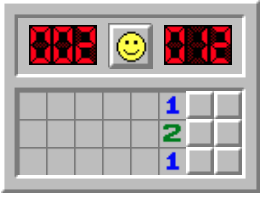
\includegraphics[width=.35\textwidth]{figures/minesweeper.png}
     \caption{Minesweeper with $N = 24$ and $M=2$}
     \label{fig:minesweeper}
 \end{figure}
Minesweeper (see Figure \ref{fig:minesweeper}), the well-known computer game, is closely related to the wumpus world. A minesweeper world is a rectangular grid of $N$ squares with $M$ invisible mines scattered among them. Any square may be probed by the agent; instant death follows if a mine is probed. Minesweeper indicates the presence of mines by revealing, in each probed square, the number of mines that are directly or diagonally adjacent. The goal is to probe every unmined square. Let $X_{i,j}$ be true iff square $\left[i, j\right]$ contains a mine. 
\begin{enumerate}
    \item Write down the assertion that exactly two mines are adjacent to $\left[1,1\right]$ as a sentence involving some logical combination of $X_{i,j}$ propositions.
    \begin{solution}
    \\
    This is a disjunction with $28$ disjuncts, each one saying that two of the neighbours are true and the others are false. The first disjunct is
    $$ X_{2,2} \land X_{1,2} \land \lnot X_{0,2} \land \lnot X_{0,1} \land \lnot X_{2,1} \land \lnot X_{0,0} \land \lnot X_{1,0} \land \lnot X_{2,0}.$$ 
    The other $27$ disjuncts each select two different $X_{i,j}$ to be true.
    \end{solution}
    \item Consider the configuration shown in Figure \ref{fig:minesweeper}. Express the constraints implied by this configuration and perform a backtracking search to determine the position of the 2 mines.
    \begin{solution}
    \\
    We will put constraints on the variables $X_{0,6}, X_{1,6}, X_{2,6}, X_{0,7}, X_{1,7}, X_{2,7}$ only, the others being obviously assigned \textbf{false}.
    Let's first express the constraints implied by each informative cell independently:
    \begin{itemize}
        \item cell 0, 5 is equal to 1: $(X_{0,6} \land \lnot X_{1,6}) \lor (\lnot X_{0,6} \land X_{1,6})$
        \item cell 1, 5 is equal to 2: $(X_{0,6} \land X_{1,6} \land \lnot X_{2,6}) \lor (X_{0,6} \land \lnot X_{1,6} \land X_{2,6}) \lor (\lnot X_{0,6} \land X_{1,6} \land X_{2,6})$
        \item cell 2, 5 is equal to 1: $(X_{1,6} \land \lnot X_{2,6}) \lor (\lnot X_{1,6} \land X_{2,6})$
    \end{itemize}
    We have also to express that there is exactly two mines: $(X_{0,6} \land X_{1,6} \land \lnot X_{2,6} \land \lnot X_{0,7} \land \lnot X_{1,7} \land \lnot X_{2,7}) \lor (\lnot X_{0,6} \land X_{1,6} \land X_{2,6} \land \lnot X_{0,7} \land \lnot X_{1,7} \land \lnot X_{2,7}) \land \left[...\right]$, where $\left[...\right]$ stands for all the $\frac{6\times5}{2} - 2$ other possible combinations of two true variables out of the six, for readability we will denote this constraint as $C_6^2$.
    Exercise at home: \textit{Put all the constraints in CNF (Conjunctive Normal Form, i.e. in a conjunction of disjunctions).}
    Applying the backtracking algorithm yields to:
    \begin{enumerate}
        \item Assign $X_{0,6} = T$
        \item Assign $X_{1,6} = F$ (first constraint)
        \item Assign $X_{2, 6} = T$ (second constraint and third)
        \item Assign $X_{0, 7} = X_{1, 7} = X_{2, 7} = F$ (Number of mines constraint)
    \end{enumerate}
    \end{solution}
\end{enumerate}

 \section*{Exercise 4: K-Knights $\star$}
 Consider the problem of placing $k$ knights on an $n\times n$ chessboard such that no two knights are attacking each other, where $k$ is given and $k \leq n^2$.
 \begin{enumerate}
     \item Choose a CSP formulation. In your formulation, what are the variables?
     \begin{solution}\\
     Solution A: There is a variable corresponding to each of the $n^2$ positions on the board.\\
    Solution B: There is a variable corresponding to each knight.
     \end{solution}
     \item What are the possible values of each variable?
     \begin{solution}\\
     Solution A: Each variable can take one of two values, \{occupied,vacant\} \\
     Solution B: Each variable’s domain is the set of squares.
     \end{solution}
     \item What sets of variables are constrained, and how?
     \begin{solution}\\
     Solution A: every pair of squares separated by a knight’s move is constrained, such that both cannot be occupied. Furthermore, the entire set of squares is constrained, such that the total number of occupied squares should be k.\\
Solution B: every pair of knights is constrained, such that no two knights can be on the same square or on squares separated by a knight’s move. Solution B may be preferable because there is no global constraint, although Solution A has the smaller state space when k is large.
     \end{solution}
 \end{enumerate}
 \section*{Exercise 5: More propositional logic $\star$}
 Given the following, can you prove that the unicorn is mythical? How about magical? Horned?\\
\textit{If the unicorn is mythical, then it is immortal, but if it is not mythical, then it is a mortal mammal. If the unicorn is either immortal or a mammal, then it is horned. The unicorn is magical if it is horned.}
\begin{solution}\\
We cannot say if the unicorn is mythical but it is definitely magical and horned.
\end{solution}

 
   \section*{Supplementary materials}
   \begin{tabular}{lc}
       \href{https://www.codeproject.com/Articles/34403/Sudoku-as-a-CSP}{Sudoku}  & \qrcode{https://www.codeproject.com/Articles/34403/Sudoku-as-a-CSP}  \\
       & \\
        \href{http://ai.berkeley.edu/sections/section_2_mA5IBOWiF6cw3yoIh65hXTiBY6mPiD.pdf}{Berkeley 1} & \qrcode{http://ai.berkeley.edu/sections/section_2_mA5IBOWiF6cw3yoIh65hXTiBY6mPiD.pdf}\\
        & \\
    \href{https://inst.eecs.berkeley.edu/~csT88/fa19/assets/section/section2.pdf}{A nice and short CSP synthesis} & \qrcode{https://inst.eecs.berkeley.edu/~csT88/fa19/assets/section/section2.pdf}
    
   \end{tabular}
\end{document}
